\documentclass[12pt]{article}
\usepackage{graphicx} % Required for inserting images
\usepackage{enumitem}
\usepackage{parskip}
\usepackage[a4paper, margin=2.54cm]{geometry}
\usepackage{amssymb}
\usepackage{amsmath}
\usepackage{bm}
\usepackage{mathptmx}
\usepackage{setspace}
\usepackage{tikz}
\usetikzlibrary{arrows.meta}
% --- APA CITATION SETUP ---
\usepackage[authoryear,round]{natbib}
\bibliographystyle{chicago}
\doublespacing

\title{Demystifying Anchoring}
\author{Shin JeongBean}
\date{}

\begin{document}
\setlength{\parskip}{8pt}
\setlength{\parindent}{1em} 
\maketitle
Brian Epstein, in his series of works \citep{Epstein2014-EPSHMK, Epstein2014-EPSSOW, Epstein2014-EPSWII, Epstein2015-EPSTAT, Epstein2015-EPSAFF}, developed an account of the generation of social facts. Roughly, according to Epstein, for a social fact $[s]$ to hold, there must be \textit{anchors} $[a_1], \dots, [a_n]$ setting up the \textit{frame principle} which specifies that $[g]$ grounds $[s]$ if $[g]$ obtains. And $[s]$ would obtain if $[g]$ obtains, for $[g]$ would ground $[s]$. He terms the ``setting up'' relation \textit{anchoring}, and further argues that anchoring is distinct from grounding.

\par
In this paper I argue that anchoring need not be a \textit{sui generis} metaphysical relation. I do not argue that anchoring is just grounding, nor that there is a single familiar metaphysical relation that could be identified as anchoring. Instead, I show that assuming any plausible modal profile for the types of anchored facts, we can find familiar metaphysical or linguistic devices which can perform the supposed work of anchoring. In particular, I examine the various possibilities of the nature of \textit{exportation} of anchoring, which has been suggested as the core reason why anchoring is different from grounding. It will be shown that given any plausible characterization of exportation, we can utilize familiar metaphysical relations to achieve theoretical purposes that Epstein wished to achieve via anchoring; and make sense of the intuition that the supposed anchors have something to do with the fact they explain. 

\par
First, I briefly summarize the theoretical motivation for anchoring and its supposed role in social ontology (\S 1.1), and the argument for the distinction between grounding and anchoring from exportation (\S 1.2). In \S 2, I discuss two extreme accounts of exportation: to no possible worlds (\S 2.1), and to all possible worlds (\S 2.2), and show that in such cases either anchoring just is grounding, or the supposed anchors merely fix the reference of a term. Thus, in \S 3 I assume anchors export to some but not all possible worlds. I then consider four exhaustive cases of exportation, where I argue that either it is impossible (\S\S 3.2, 3.3) or it leads to the conclusion that anchoring is not \textit{sui generis} (\S\S 3.1, 3.4). 
%==============================================
\section{Anchoring and Exportation}
\subsection{Anchoring in social ontology}
%==============================================
The notion of \textit{anchoring} is originally motivated by the observation that there are two different kinds of individualism in social ontology, each claiming that social facts are somehow entirely ``built from'' facts about individual people \citep{Epstein2014-EPSWII,Epstein2015-EPSTAT}. The first, \textit{grounding individualism}, in its strongest form, is the thesis that all social facts are fully grounded in facts about individuals. This is implausible: among the indispensable grounds of [a slice of ham is unkosher]\footnote{
    I use square brackets ``[\dots]'' to express the fact that \dots. For readability, I also use bracketed variables such as [$p_1$], [$p_2$] for facts. 
} are [a slice of ham is made from a pig] and [pigs are cloven-hoofed but do not chew their cud], neither of which seems to be a fact about individuals.


\par
But one may still insist that the social world is \textit{set up} by facts about individuals---their collective acceptance, regular behaviors, mutual beliefs, and so on. Given that a social fact $[s]$ is fully grounded in $[g]$, we may ask why $[s]$ is such that it can be grounded in $[g]$. Epstein answers, following \citet{Searle1995-SEATCO}, by supposing there are rules or principles that govern what kinds of facts ground the given kind of facts, namely, \textit{frame principles}. Typically, a frame principle governs the grounding condition of facts about something falling into a certain kind, or having a certain property. In the example of unkosher foods, the relevant frame principle would be $\forall x$(\{[$x$ \textit{is a food made from} $F$], [$F$\textit{s are cloven-hoofed animals that do not chew their cud}]\} \textit{grounds} [$x$ \textit{is unkosher}]).\footnote{
    If one wishes, a frame principle can be regarded as a \textit{generic grounding fact}: \textit{what it is to be X} grounding \textit{what it is to be Y}. See \citet{Fine2015-FINUFF}.
} \textit{Anchoring}, then, is a ``setting up'' relation between a frame principle and some facts---namely, its \textit{anchors}--- which is different from the grounding relation. Plausibly, the anchors for the frame principle about something being an unkosher food would include facts about the content of the Bible, and its authority in Judaism, and so on. 

\par
\textit{Anchoring individualism}, which captures the idea that the social world is set up by individualistic facts, is the thesis that all anchors should be individualistic facts. It is compatible with the denial of grounding individualism. One can agree that [pigs are cloven-hoofed animals that do not chew their cud] partially grounds [a slice of ham is unkosher], but insist that the relevant frame principle is anchored fully by individualistic facts: for example, facts about each person having a certain kind of acceptance towards the principle \citep{Searle1995-SEATCO}, or their having mutual beliefs and regularities in behavior \citep[Book~3]{Hume1978-SELTOH-3}.\footnote{One of the main enterprises of \citet{Epstein2015-EPSTAT} is to refute anchoring individualism. For reply, see \citet{Francesco2016-FRAEOA-10}.}

\par
The introduction of the notion of anchoring primarily serves the function of distinguishing anchoring individualism from grounding individualism. Yet Epstein argues that anchoring has other metaphysical roles as well. One thing is to provide a non-causal metaphysical reason why a frame principle, and the social fact grounded according to it, hold (Epstein, \citeyear{Epstein2015-EPSAFF}; see also Schaffer, \citeyear{Schaffer2019-SCHAAG-5}). It is easy to see that frame principles are explicable in terms of their anchors. We can partially explain the frame principle for being unkosher in terms of the content of \textit{Leviticus}, which supposedly anchors it. Moreover, Epstein takes the obtaining of a social fact to be partially explained via the grounds \textit{and} the frame principle which gives such a grounding condition. But then, since the frame principle is explicable in terms of its anchors, they should also be capable of partially explaining the social fact in question. 

\par
Another function of anchoring is to provide an account of why a given social kind has the nature it has in a somewhat non-arbitrary way \citep{Epstein2014-EPSHMK,Epstein2025-EPSSOQ}. We can, of course, define a new kind however we want. For example, let us define a kind \textit{Schmoller} as follows: for any $x$, [$x$ is a Schmoller] is fully grounded in either [$x$ is printed by BEP (in a such-and-such way)] \textit{or} [$x$ is drawn by a 7-year-old kid (in a such-and-such way)]. But the kind \textit{Schmoller} is not distinctive as a social kind, in the sense that the kind \textit{Dollar} is. According to Epstein, \textit{Dollar} is distinctive in the sense that it is socially constructed whereas \textit{Schmoller} is not; and to be socially constructed is to have social anchors. While the frame principle about something being a Dollar is anchored by, say, the relevant federal laws and the government institution, the frame principle about something being a Schmoller, if there is one, does not have such social anchors. 

\par
In sum, anchoring is introduced to serve the following purposes:
\begin{itemize}
    \item[(A1)] To distinguish between two kinds of individualism in social ontology;
    \item[(A2)] To identify the non-causal metaphysical reason for the obtaining of frame principles about some social facts;\footnote{
    Strictly speaking, Epstein argues that facts and frame principles other than those in the social world can also admit of anchors \citep[see especially][]{Epstein2019-EPSAVG}. However, the notion of anchoring has been applied almost exclusively within social ontology. Thus, in what follows I will focus solely on the role of anchoring in the field of social ontology. 
}
    \item[(A3)] To explain how a social kind is socially constructed to have the nature it has.
\end{itemize}
In other words, in arguing that anchoring is not \textit{sui generis}, I must show how familiar devices can do the work of anchoring. Yet it should first be examined why anchoring was suggested to be a novel metaphysical tool. 

\subsection{Grounding-anchoring monism and exportation}

The general scheme of the generation of social facts, according to Epstein, is as follows. First there are \textit{anchors} $[a_1], [a_2], \dots$ setting up a frame principle $FP$, which specifies that $[g_1], [g_2] \dots$ would fully ground the social fact $[s]$ if they obtain. Second, given that $[g_1], [g_2] \dots$ obtain, they ground $[s]$. In a diagram:

\begin{center}
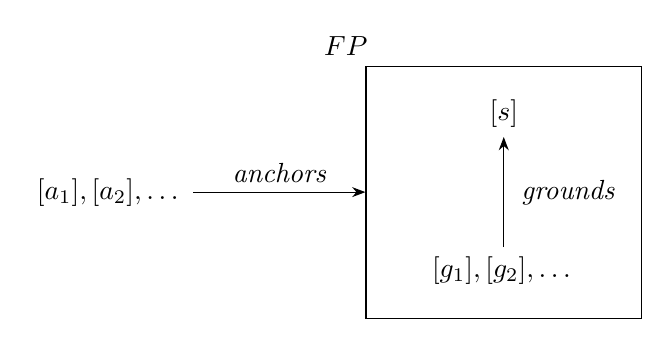
\begin{tikzpicture}[font=\itshape, >=Stealth]

% box for the frame principle (FR)
\node[draw, minimum width=3.5cm, minimum height=3.2cm, label={[font=\itshape]above left:$FP$}] (box) at (4,0) {};

% contents of the box: [s] on top, grounds arrow, [g1],[g2],... below
\node (s) at (4,1) {$[s]$};
\node (g) at (4,-1) {$[g_1],[g_2],\dots$};
\draw[->] (g) -- (s) node[midway, right, xshift=0.1cm] {grounds};

% anchors, to the left, pointing into the box
\node (a) at (-1, 0) {$[a_1],[a_2],\dots$};
\draw[->] (a) -- (box.west) node[midway, above] {anchors};

\end{tikzpicture}
\end{center}
An important feature of the anchoring framework is that the anchoring relation, viz., the relation between $[a_1], [a_2], \dots$ and $FP$, is different from the grounding relation, viz., the relation between $[g_1], [g_2], \dots$ and $[s]$. Let us term this view ``\textit{grounding-anchoring dualism}'' (simply ``dualism'' below).

\par
Notice, however, (A2) seems to hardly support the claim that anchoring is \textit{sui generis}. Grounding, if not anything, can do exactly the same job of providing a non-causal metaphysical reason for something. As \citet{Schaffer2019-SCHAAG-5} argues, in this respect ``anchoring does as grounding does''. This motivates \textit{grounding-anchoring monism} (simply ``monism'' below): that there is only one relation in operation when generating social facts. 

\par
A prevalent form of monism suggests that $[a_1], [a_2], \dots$, together with $[g_1], [g_2], \dots$ fully ground $[s]$.\footnote{``Conjunctivism'', in \citet{Epstein2015-EPSTAT}'s term; \citet{Hawley2019-HAWCOB-4}, \citet{Pagano2023-PAGSCS} and \citet{Chilovi2026-CHIAGA-3} follow this usage. \citet{Schaffer2019-SCHAAG-5} terms the same idea  ``Grounding-Only view'', whereas \citet{Chilovi2026-CHIAGA-3} uses the term in a broader sense. Everyone mentioned in this footnote except Epstein defends the view that $[a_1], [a_2], \dots$ also ground $[s]$.} In a diagram: 

\begin{center}
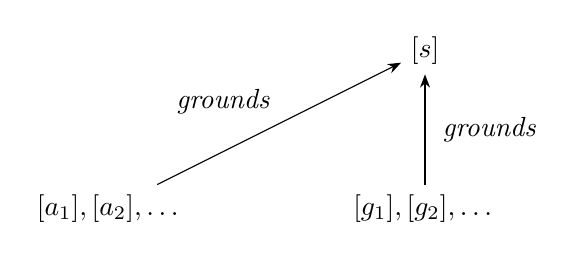
\begin{tikzpicture}[font=\itshape, >=Stealth]


% contents of the box: [s] on top, grounds arrow, [g1],[g2],... below
\node (s) at (4,1) {$[s]$};
\node (g) at (4,-1) {$[g_1],[g_2],\dots$};
\draw[->] (g) -- (s) node[midway, right, xshift=0.1cm] {grounds};

% anchors, to the left, pointing into the box
\node (a) at (0, -1) {$[a_1],[a_2],\dots$};
\draw[->] (a) -- (s) node[midway, above left] {grounds};

\end{tikzpicture}
\end{center}

Let us term this view ``\textit{conjunctive monism}''. While this has been more popular among monists, this is not the only reasonable framework under monism. Instead, one can hold that the supposed anchors ground $[[g_1], [g_2], \dots$ fully ground $[s]]$, or perhaps simply [$FP$ obtains].\footnote{A similar view is developed by \citet{Passinsky2025-PASSCA-2}.} Again, in a diagram:

\begin{center}
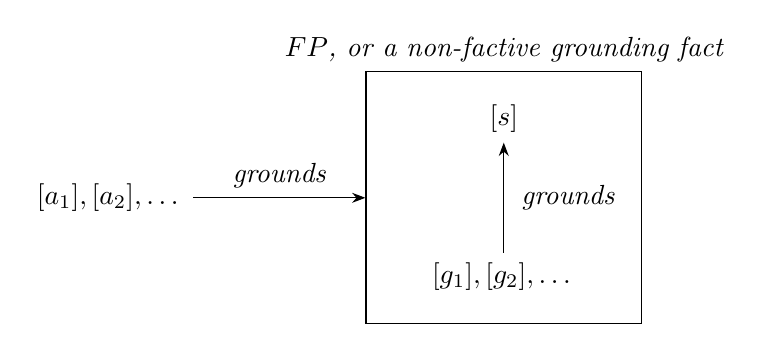
\begin{tikzpicture}[font=\itshape, >=Stealth]

% box for the frame principle (FR)
\node[draw, minimum width=3.5cm, minimum height=3.2cm, label={[font=\itshape]above:$FP$, or a non-factive grounding fact}] (box) at (4,0) {};

% contents of the box: [s] on top, grounds arrow, [g1],[g2],... below
\node (s) at (4,1) {$[s]$};
\node (g) at (4,-1) {$[g_1],[g_2],\dots$};
\draw[->] (g) -- (s) node[midway, right, xshift=0.1cm] {grounds};

% anchors, to the left, pointing into the box
\node (a) at (-1, 0) {$[a_1],[a_2],\dots$};
\draw[->] (a) -- (box.west) node[midway, above] {grounds};

\end{tikzpicture}
\end{center}
Let us term this view ``\textit{meta-ground monism}''. Two kinds of monism account for (A1) and (A3) in different ways. For meta-ground monism, it is more straightforward. The distinction between grounding individualism and anchoring individualism simply becomes the distinction between individualism about what grounds a social fact, and individualism about what grounds \textit{that} grounding fact in turn. Moreover, under meta-ground monism, how a social kind is socially constructed to have the nature it has can simply be explained by the social grounds of the frame rule about itself. 

\par
Conjunctive monists can distinguish two kinds of individualism by acknowledging that there are `rule-setting' grounds and `move-making' grounds \citep[760--1]{Schaffer2019-SCHAAG-5}. Thus, there are two different kinds of individualism---individualism about rule-setting grounds on the one hand, individualism about move-making grounds on the other. If the distinction between two sorts of grounds is intelligible, one can further suggest that a kind is socially constructed if it has social facts as its rule-setting grounds.\footnote{Some exportation scenarios will be consistent with both, some others only with meta-ground monism, and still others inconsistent with either monism. Still, in this paper, I do not discuss which monism is favorable under the scenarios that are consistent with both of them.}

\par
\citet{Epstein2015-EPSTAT,Epstein2019-EPSAVG}, however, argues that it is precisely (A2) that supports dualism, since the non-causal metaphysical reason for the obtaining of frame principles seems to manifest different modal behaviors from grounding. 



\bibliography{refs} % Make sure 'refs.bib' exists in the folder
\end{document}